\begin{frame}
  \frametitle{DG-FEM Notation}
  \begin{columns}[t]
    \begin{column}{0.6\textwidth}
      \begin{block}{Interface facets}
        \begin{center}
          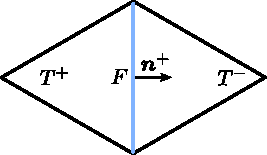
\includegraphics[scale=1.0]{pdf/dg-terms-interface.pdf}
          \\
          \vspace{-2em}
          \begin{alignat*}{2}
              \text{\colemph{Average} } &\avg{v} = \tfrac{1}{2}(v^+ + v^-)
            \\
            \text{\colemph{Jump} }      &\jump{v} = (v^+ - v^-)
          \end{alignat*}
%          $\jump{v} \bfn $ independent of orientation of $\bfn^+$
        \end{center}
      \end{block}
    \end{column}
    \begin{column}{0.4\textwidth}
      \begin{block}{Boundary facet}
        \begin{center}
          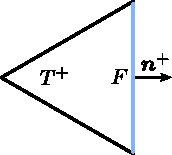
\includegraphics[scale=1.0]{pdf/dg-terms-boundary.pdf}
          \\
          \vspace{-2em}
          \[
            \avg{v} = \jump{v} = v
          \]
        \end{center}
      \end{block}
    \end{column}
  \end{columns}
  {\colemph{Jump identity}}
  \begin{equation*}
    \jump{(\nabla_h v) w_h } = \jump{\nabla_h v} \avg{w_h} 
    + \avg{\nabla_h v} \jump{w_h}
  \end{equation*}
\end{frame}
